\documentclass[review, authoryear]{elsarticle}

\usepackage{custom-local-els}

\journal{Journal of Network and Computer Applications}

\begin{document}  

\begin{frontmatter}

\title{Simulations for Power Analysis and Study Design: do Lab Animal Findings
About the Gompertz-Makeham Model Extend to Human Populations?}

\author[deb]{Alex F. Bokov\corref{cor1}}
\ead{bokov@uthscsa.edu}
\author[deb]{Jonathan A. Gelfond}
\author[deb]{Alfredo Tirado-Ramos}
\author[um]{Scott D. Pletcher}

\cortext[cor1]{Corresponding author}


\address[deb]{UT Health, San Antonio}
\address[um]{University of Michigan, Ann Arbor}


\begin{abstract}
In clinical trials as well as in basic research, critical decisions
about experimental design need to be made in advance, often when little
is known about the population being studied. Effect sizes, variability,
and other statistical properties are not reliably portable from one
study population or research topic to another. By definition, the more
novel an experiment is the fewer `similar' previous experiments it can
draw on the the more acute this problem. We have extended our earlier
survival simulation work from laboratory rodents to human populations.
Moreover we generalized from a two dimensional parameter space to three
dimensions in order to determine whether or not the Gompertz-Makeham
model has any advantage over simpler and more commmonly used survival
models.
\end{abstract}

\begin{keyword}
survival analysis, predictive modeling, statistics
\end{keyword}

\end{frontmatter}

\section{Introduction}\label{introduction}

In planning an experiment in basic or clinical research, power analysis
is important for determining feasibility and budgeting for a sample size
sufficient to avoid an indeterminate result. Conversely, accurate power
analysis also helps contain costs by avoiding excessive sample sizes.
Power analysis depends on a probability density function over all
possible outcomes for an experiment given a particular set of
parameters. Real-world processes, especially in the life sciences, often
have density functions that either lack a closed-form solution or are
complex to implement. Furthermore, it is not always clear how large of a
sample size is sufficient to meet the asysmptotic assumptions of one's
statistical tests. A promising approach is to generate simulated data
spanning the relevant parameter-space.

This allows the researcher to realisticall budget for follow-up
intervals, participant recruitment targets, and choice of analysis
method prior to initiating an experiment or clincal trial.

Existing Monte Carlo methods to characterizing distributions
\citep{fang08, schoemann14} depend on hardcoded assumptions about the
type of phenomenon being studied and the statistical model being fitted
to the data. We have developed and are continuing to improve an open
source library for the R statistical language that implements a
simpulation and test framework that can be adapted to various
populations, study designs, and outcomes being measured. Instead of
interpreting treatement effect as a simplistic uni-directional
difference our approach is to accrue data by repeatedly running
statistical workflows and decision rules representative of what the
researcher is considering for their actual experiment. These virtual
experiments are imlemented as modules with a automated code-generation
function that makes it easier to create new ones or adjust existing ones
to the needs of a given project.

\section{Background}\label{background}

In mammals, the risk of mortality is not constant over time. Rather, it
increases log-linearly with age
{[}\citet{MuellerGompertzequationpredictive1995};
FinchSlowmortalityrate1990{]}. Using only ages of death or at
loss-to-followup (censored events), the Gompertz probability density
function can be used to obtain the maximum likelihood estimates for the
initial risk of mortality (IMR or \(\lambda\) ) and the rate at which it
accelertates (RoA or \(\gamma\) ). On a log scale these correspond to a
slope and an intercept of mortality risk over time. These parameters can
then be plugged back into the observed data to its likelihood. When
comparing a test group with a control group the null hypothesis is that
their lifespans are no different from each other and therefore the same
pair of IMR and RoA parameters are sufficient to fit the observed data.
However, if the two groups have different IMRs, a model with three
parameters-- IMR\(_{control}\), IMR\(_{treated}\), and RoA -- will have
a larger likelihood and this is the basis of the likelihood ratio test
as used here. The same principle applies a difference in the RoAs
between the groups, or differences in both parameters (now the
likelihood from the two-parameter null model is being comparted to the
likelihood from a four-parameter model where everything is different
between the two groups, adjusted for the additional difference in
degrees of freedom).

We recently reported that the Weibull and the Cox Proportional Hazard
tests had roughly similar performance to a likelihood ratio test using
estimates of Gompertz model parameters obtained via Nelder-Mead
optimization \citep{NelderSimplexMethodFunctionMinimization1965}. The
Weibull model was found to be slighly less sensitive and slightly more
resistant against false positives than the others
\citep{bokov2017riskmodels}. However, when the IMR increased
(i.e.~higher initial hazard) and RoA decreased (i.e.~hazard increases
more slowly) in a test group compared to the control group, or vice
versa, only the Gompertz likelihood ratio test could detect differences
even though the survival curves visibly diverged. Our simulations were
based on hazard estimates for laboratory mice.

But we cannot assume that these conclusions are automatically applicable
to humans. Clearly humans are orders of magnitude longer-lived so human
IMR and RoA parameters will be smaller and harder to detect.
Furthermore, laboratory animals are kept in as homogeneous an
environment as possible, while humans are in some sense a `wild'
population so in addition to IMR and RoA, a third parameter may need to
be included to account for extrinsic hazards-- EH, or \emph{c} . This
extended model is called Gompertz-Makeham and was used here.

\section{Methods}\label{methods}

\subsection{Data}\label{data}

In our earlier work we used combined results for just the control groups
of multiple longevity studies carried out using non-mutant C57Bl6 mice
to obtain parameters with which to generate simulated data
representative of this species. For humans we used life-tables for the
combined US population from 2013 \citep{arias_united_2017b}. These are
the second to most recent available, and we are deliberately holding out
the 2014 installment published this year \citep{arias_united_2017b} as a
validation dataset for upcoming work.

The life table data is in one-year increments for 99,316 individuals
with all deaths over 100 years binned together. We extracted these data
out into individual time-points and smoothed out the bins to monthly
bins rather than yearly, with all deaths above 100 years given a
censoring indicator. In Figure 1 we present the raw data and the
smoothed data on the same scale, along with a simulated survival curve
generated using the parameters estimated from this data (IMR =
3.024956e-06, RoA = 7.669709e-03, and EH = 1.970425e-05). It can be seen
from the figure that smoothing the time intervals to months (necessary
to avoid numeric artifacts caused by too many tied events) does not
significantly bias the data. It also shows how closely the simulated
distribution of deaths resembles the real data, though the only
information from the data that was used by the simlation were the three
hazard parameters.

\begin{figure}
\centering
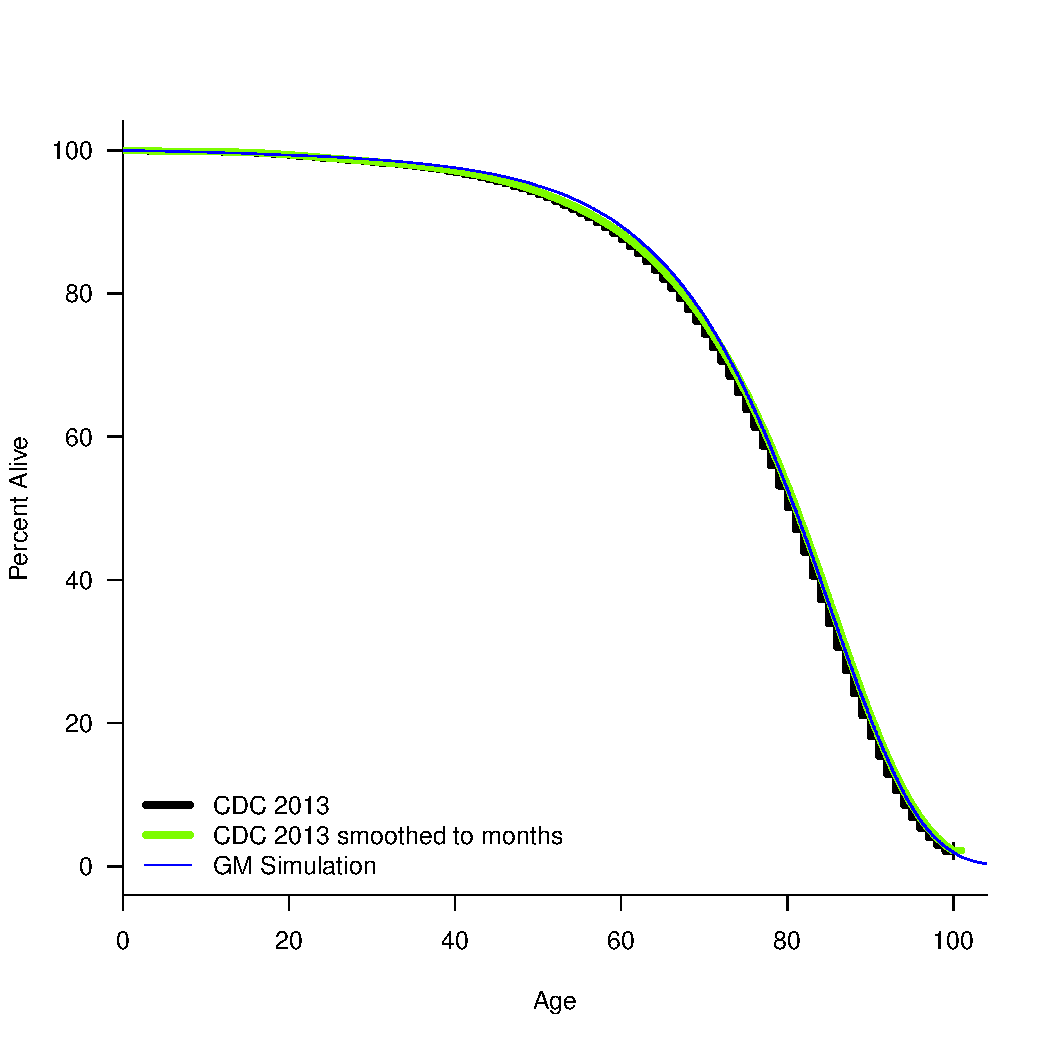
\includegraphics[width=0.50000\textwidth]{pt2017_figure01.pdf}
\caption{Real, smoothed, and simulated human survival data.}
\end{figure}

In our rodent results \citep{bokov2017riskmodels} we found that below a
sample size of 60, there was an increasing bias in the estimates of both
the IMR and RoA parameters. In order to find the corresponding threshold
for humans we used the above parameter estimates to create 100,000
simulations of this cohort, varying the sample size between 100 and 500.
For each sample we estimated the three Gompertz-Makeham parameters and
compared to the known values used by the simulation in order to assess
how variability and estimation bias changes with sample size. We found
the threshold for a human population binned into 1-month intervals to be
200. (Figure 2.)

\begin{figure}
\centering
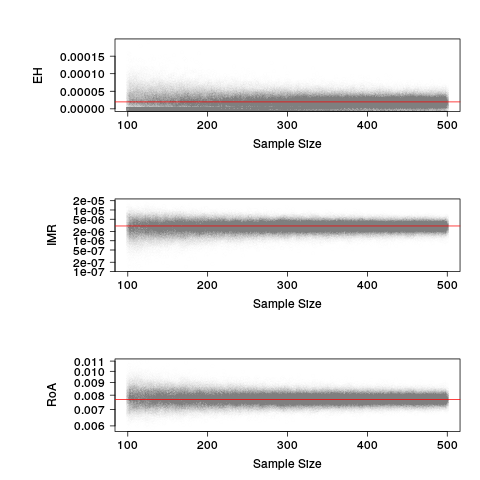
\includegraphics[width=0.60000\textwidth]{pt2017_figure02.png}
\caption{Variance and bias versus sample size. For IMR and RoA the y
axis is on the log scale.}
\end{figure}

\subsection{Software}\label{software}

Our simulation framework for power analysis and exploration of
distributional properties of data is called PowerTrip (
https://github.com/bokov/powertrip/tree/test\_polar ). It is implemented
as a package for the R statistical language
\citep{Rlanguage, survival-package, survival-book} and has the following
other packages as its essential dependencies: eha \citep{eha}, MASS
\citep{MASS}, SparseM \citep{SparseM}, and broom \citep{broom}. Some of
the figures in this manuscript were prepared using the plot3D
\citep{plot3D} and rgl \citep{rgl} packages.

At initialization, the user sets upper and lower bounds on all model
parameters, and the reference parameters that will be used to simulate
the control group for every comparison. The parameter-space is centered
on the reference point and treatment effects are modeled as deviations
from it. Here, the parameter deviations the three hazards: IMR, RoA, and
EH. An increase in any of them would result in a shorter survival time
relative to the control group, \emph{ceteris paribus}. Likewise a
decrease would be associated with a longer survival-time. One of the
distinguishing features of our approach is that instead of making
assumptions about the direction of change due to an experimental
intervantion, we probe every possible direction and continuously update
our estimate of the multi-dimensional surface that represents the
combinations of paramter differences that are jointly large enough to be
detectable by the proposed statistical method/s (or more generally,
decision algorithm/s) at the specified detection rate (here we picked
the 80\% resolving power typical in the life sciences).

The bounded parameter space (on the log scale) is uniformly sampled.
Here we used 150 points each round. The Cartesian coordinates are
converted to polar coordinates and the radial coordinate \emph{r} is
ignored. At each of set of angles \(\phi_{i1,\dots,in}\), random radial
distances are sampled from a \emph{B(1.333,1)} distribution (which we
empirically found to mitigate some of the bias toward sampling too close
to the origin). Each of these values of \emph{r} along the angle
\(\phi_{i1,\dots,in}\) is converted back to relative Cartesian
coordinates and passed to a module that interprets them (in our case) as
IMR, RoA, and EH. This module simulates a dataset representing a control
group and a treatment group with those differences from the control
group's hazards. This dataset is passed to a panel of decision modules,
each of which evaluates the same dataset and returns a TRUE/FALSE
response which in our case indicates whether or not the statistical test
wrapped by this module rejected the null hypothesis of no difference
between the two groups.

\emph{There are no hardcoded assumptions about the module that simulates
the data, nor the modules that analyze it and return decisions.} In
fact, we have a function (\texttt{new.ptpnl()}) that accepts code
snippets from the researcher to specify the analysis method, the
decision rule, and a logging/summary function. It then dynamically
generates an analysis module that correctly hooks these pieces into
\texttt{powertrip()}. We also extended native R's \texttt{update()}
mechanism to provide a simpler alternative to make minor changes to
existing analysis modules. As a proof of concept, alongside the survival
analysis we are reporting here, we wrote a simulator module that
generates multivariate regression datasets with interaction terms and an
accompanying panel of two linear model wrappers-- one that includes
interaction terms and one that attempts to detect inter-group
differences using only additive terms. The boundaries of their
respective 80\% detection regions are shown in figure 3.

\begin{figure}
\centering
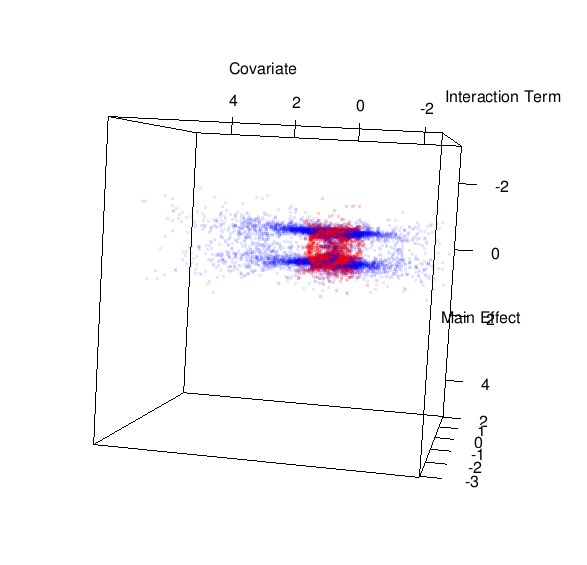
\includegraphics[width=0.50000\textwidth]{pt2017_figure03.png}
\caption{Using PowerTrip for multivariable linear regression. The blue
points indicate a main effects only model. Both models can detect
additive differences between the groups (i.e.~the intercept) but
regardless of the size of the interaction term (i.e.~the slope of the
covariate being different between treatment and control), the additive
model cannot detect it. The model with interactions can, and as a result
its detection surface extends in all directions.}
\end{figure}

Powertrip is designed to allow multiple `competing' analysis modules to
evaluate the same simulated dataset allowing for the fairest possible
comparison of sensitivity, precision, bias, and any other aspect of
performance that is of interest to the researcher. After all analysis
modules have evaluated the dataset simulated at each point along
\(\phi_{i1,\dots,in}\), a univariate logistic regression model is fitted
for each analytic module, where the vector of TRUE/FALSE responses from
the model is the outcome variable and the corresponding \emph{r} is the
predictor (since the \(\phi_{i1,\dots,in}\) is held constant). The
\texttt{dose.p()} function from the MASS package \citep{MASS} is used to
reverse-predict the value of \emph{r} that would result in an 80\%
detection rate (i.e.~a power of 0.8). A new set of \emph{r} s is sampled
from a smaller range based on the confidence intervals of the reverse
prediction. This is the innermost loop of the process implemented by the
\texttt{phi\_radius()} function. It continues the cycle of simulation,
analysis, and prediction continues until every analysis module in the
panel either has a confidence interval within the user-specified number
of standard deviations or has undergone convergence failure. For the
non-failing modules their respective final predictions \(r_{im final}\)
are recorded as the estimates closest to the 80\% detection rate at
\(\phi_{i1,\dots,in}\). Then, \texttt{powertrip()} invokes
\texttt{phi\_radius()} for the next set of angles,
\(\phi_{(i+1)1,\dots,(i+1)n}\). After this middle loop iterates over all
the \(\phi\) s, the outer loop (also in \texttt{powertrip()}) generates
the next set of random Cartesian coordinates. But, on all iterations
after the first, at this point a \emph{second} set of predictions is
done, this time with the \(\phi\) s as the predictors and the \emph{r} s
as the outcomes. Prediction confidence intervals are harvested for each
of the newly generated \(\phi\) s. Where they are narrower than the the
overall user-defined boundaries of the parameter-space, they are used in
their stead, to further speed up convergence.

\subsection{Statistics}\label{statistics}

We used the Weibull ( \texttt{survreg(Surv(tt)\textasciitilde{}group)} )
and Cox proportional hazard (
\texttt{coxph(Surv(tt)\textasciitilde{}group)} ) models, each in a
side-by-side comparison with a likelihood ratio test comparing the fit
of a three-parameter Gompertz-Makeham model (i.e.~one set of IMR, RoA,
and ER hazards shared between the control and treatment groups ) to a
six-parameter one (i.e.~potentially each of the hazards is different).
The significance threshold was set at p\textless{}0.05.

\subsection{Other design features of
interest}\label{other-design-features-of-interest}

R normally passes variables by value, not by reference although in
recent versions lazy evaluation has made this less of a performance
issue. Nevertheless, when this much data is being moved around, it is
desirable to avoid copying entire data structures. Instead, an special
type of object that in R is called an \texttt{environment} is passed
around. It is a pointer to a container of arbitrarily large data
structures and most of the important accessor and mutator methods for
\texttt{lists} (R's workhorse data structure) also exist for
\texttt{environment} s. Results from the inner loop are logged to an
environment object and when functions in the outer loops need to access
those results they can do so without them being explicitly passed to
them. Upon completion of the run, the environment is saved to an
\texttt{.rdata} file and we have a function called
\texttt{read\_ptenv()} that can turn it into a custom object that has
its own \texttt{{[}} (subset), \texttt{print()} and \texttt{summary()}
methods that allow the researcher to cleanly and concisely retrieve from
it various combinations of variables in tabular form for analysis,
reporting, and visualization. Since state information is also stored in
this environemt object, we can restart a previously interrupted run of
\texttt{powertrip()}, or we can have one instance of
\texttt{powertrip()} complete its burn-in cycle and then launch multiple
instances from its save-file. The more collected data a
\texttt{powertrip()} instance has access to, the better its prediction
intervals will presumably be, prompt synchronization of results is not
required. Therefore in principle it is possible for multiple nodes to
constantly improve each other's performance by exporting and merging
results on a best-effort basis.

The other feature which seems to be lacking in the R packages we are
aware of are runtime hooks for debugging, saving, and even patching.
\texttt{phi\_radius()} checks its directory for the existance of files
having a user-configurable name. The \texttt{savetrigger} file causes it
to immediately save the logging environment to a file, after which the
file is removed. The \texttt{debugtrigger} file drops PowerTrip into an
R debugger without terminating it and after the debug session is
finished it can continue on as normal. Finally, if the
\texttt{sourcepatch} file is detected it is executed as an R script
within the local scope and then renamed. Prudent use of these features
reduce time wasted relaunching a lengthy process just to fix a minor
configuration error or losing data because the process has not completed
before a system shutdown. In point of fact, even though there are
convergence criteria for individual points, we don't consider the
overall simulation to ever be complete-- we intend for them to run
continuously and generating ever more precise estimates.

\section{Results}\label{results}

\subsection{Is the Makeham parameter detectable and practically
relevant?}\label{is-the-makeham-parameter-detectable-and-practically-relevant}

We have found the same inverse relationship between RoA and IMR as in
the mouse data \citep{bokov2017riskmodels}. However with these data
there was hardly any separation between the Gompertz-Makeham model and
the Weibull model in figures 4-6 below. The same pattern was observed
for the Cox proportional hazard model (not shown).

\begin{figure}
\centering
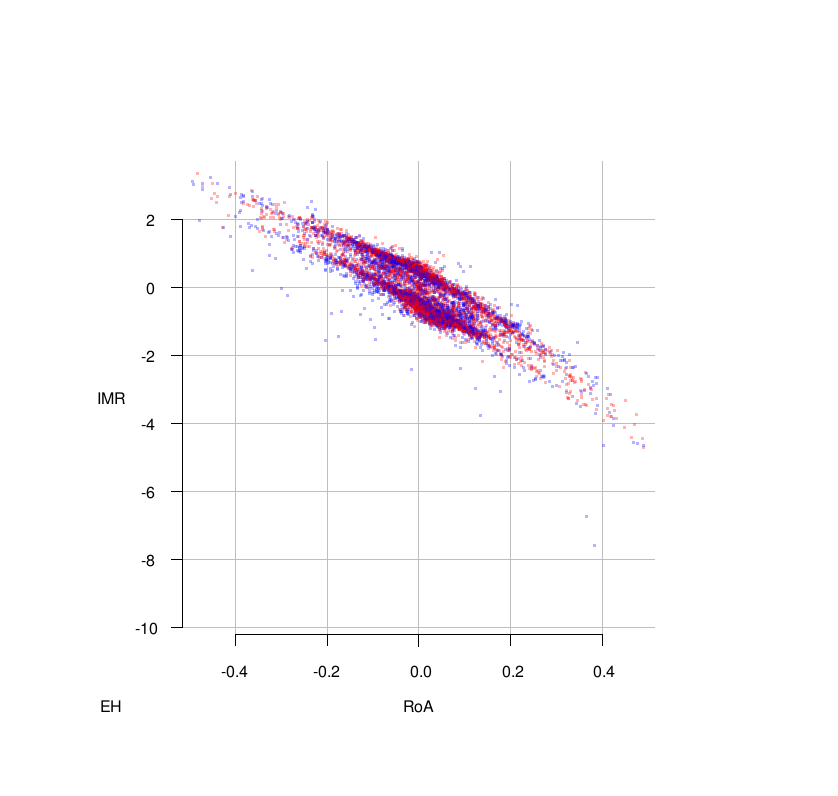
\includegraphics[width=1.00000\textwidth]{roa_vs_imr.png}
\caption{Rate of hazard acceleration versus initial hazard. Red
represents parameters differences relative to the center that are
detectable 80\% of the time by likelihood ratio test on estimated
parameters and blue represents the same for the Weibull test.}
\end{figure}

There is no linear relationshp between EH and either of the other
prameters, i.e.~perturbing the EH does not globally increase or decrease
the ability to detect differences in the other parameters. The visual
patterns in figures 5 and 6 may be illusory, due to points still being
sampled more often near the center.

\begin{figure}
\centering
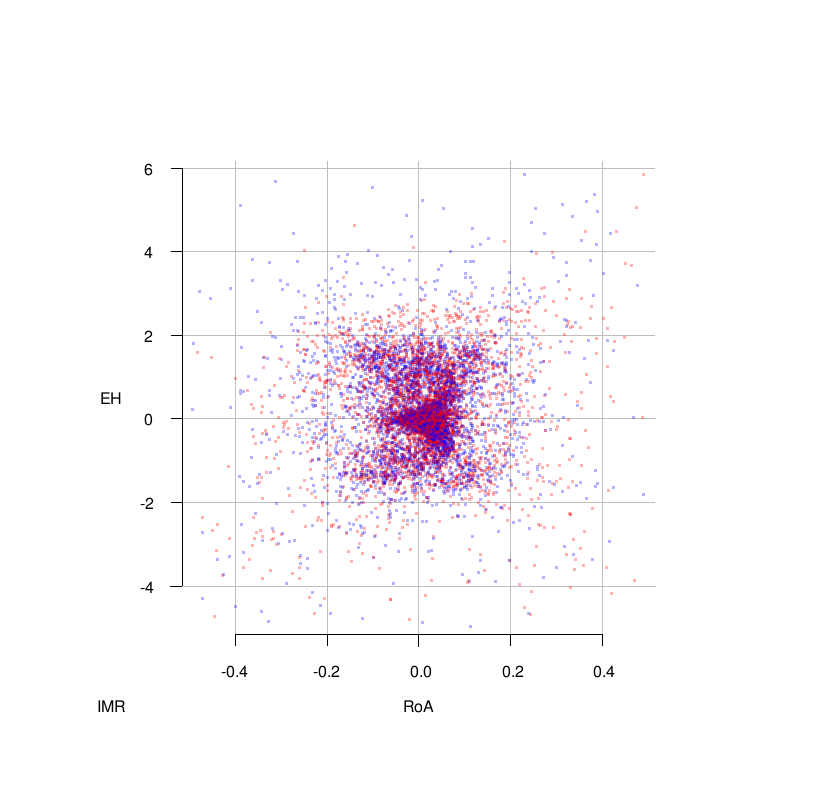
\includegraphics[width=1.00000\textwidth]{eh_vs_roa.png}
\caption{Rate of hazard acceleration versus external hazard. Red
represents parameters differences relative to the center that are
detectable 80\% of the time by likelihood ratio test on estimated
parameters and blue represents the same for the Weibull test.}
\end{figure}

\begin{figure}
\centering
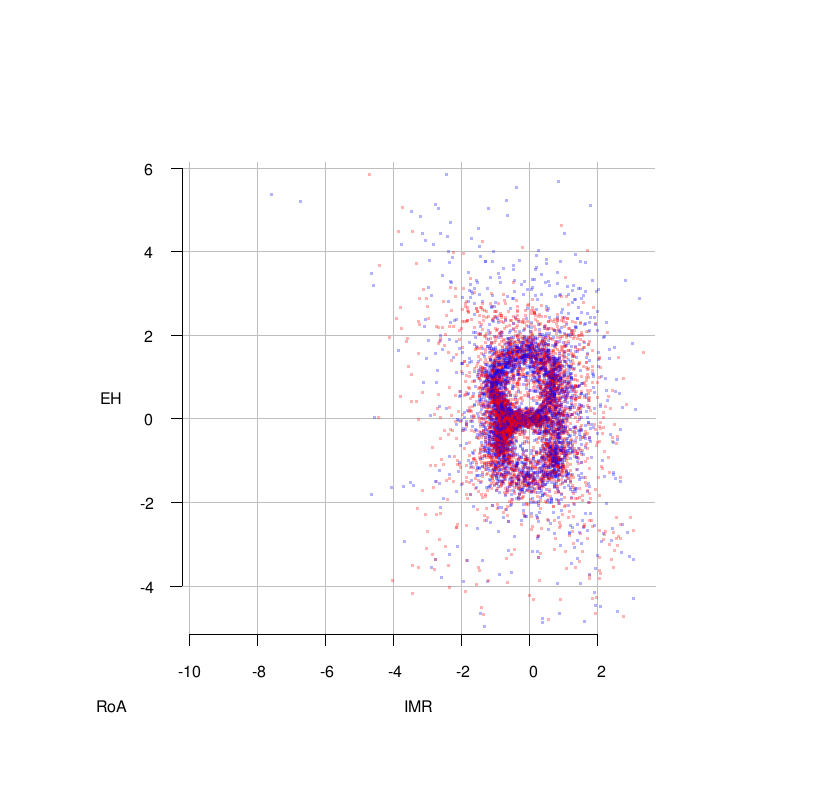
\includegraphics[width=1.00000\textwidth]{eh_vs_imr.png}
\caption{Initial mortality rate versus external hazard. Red represents
parameters differences relative to the center that are detectable 80\%
of the time by likelihood ratio test on estimated parameters and blue
represents the same for the Weibull test.}
\end{figure}

\section{Future work}\label{future-work}

\subsection{Targeting informative
spaces}\label{targeting-informative-spaces}

For predictions, there is much room for imporvement beyond just better
targeting of sampling ranges for radii. It should be possible to predict
the detection rates for the points that are sampled on the Cartesian
space in the outer loop, and target the ones that are closest to the
target distance and yet have the largest prediction confidence intervals
because they will be the most informative and impactful. This will
likely involve Kriging or inverse weighted distance interpolation and
that, in turn, requires retaining not only summaries and final estimates
for each \(\phi_{i1,\dots,in}\) but each of the indvidual points. With
improved hardware and the use of performancre optimized
\texttt{data.table} objects in R this is a likely next step.

With a good way of predicting individual points, it will become possible
for researchers to benefit from the existence of PowerTrip without
necessarily themselves having to run an instance: the fitted model
objects can be exported from an instance and used as a static prediction
engine. The role of PowerTrip then becomes that of a model factory that
continues to generate and distribute updated and more accurate model
objects.

\subsection{Modeling attrition and
recruitment}\label{modeling-attrition-and-recruitment}

Though long-term survival studies are important, they are not
representative of the most common use cases in design of human trials. A
more realistic model would be one where subjects who survive to a
particular age-range are randomly enrolled into a cohort, some of them
are randomly lost to follow-up, and the entire expriment ends after two
or three years. Notwithstanding the fact that our implementations of
these models do support right-side censoring, we have no idea what
distributional properties will be of Gompertz or Gompertz-Makeham
variables filtered through this additional selection/attrition process,
and whether a tractable closed-form probability density function exists.
But we will be able to directly perturb simulated populations that we
have demonstrated are highly similar to real ones and product conditions
more representative of clinical trials.

\subsection{Censoring and sample size as part of the parameter
space}\label{censoring-and-sample-size-as-part-of-the-parameter-space}

Since our earlier publication \citep{bokov2017riskmodels} we have
generalized our software to support an arbitrary number of model
parameters. There is no particular reason that sample size and censoring
rate cannot be added as fourth an fifth dimensions. For sample size in
particular, this would mean that instead of separate runs for finding
the ``detection surface'' for a few sample sizes and trying to guess
about what happens inbetween, we would be able to run a 4- or
5-dimensional PowerTrip that is learning a little bit about every sample
size all the time, and borrowing information from one to make
predictions about others, just as in effect here we are borrowing
information about the different parameters within the model to
accelerate convergence.

\section*{Acknowledgments}\label{acknowledgments}
\addcontentsline{toc}{section}{Acknowledgments}

This work was supported by NIH grants 1P30AG044271-01, 5T32AG021890,
2P30AG013319, and RC2AG036613.

\bibliography{paper}{}
\bibliographystyle{elsarticle-harv}

\end{document}
